\chapter{Discussion}

In this section, i will discuss what the solution that i have tried to apply and what are the difficulties and the challenges that i encountered and the unexpected challenges that i found during this implementation.

Fist after noticing that the Container having issues receiving the files, i decided to write a external script for the Container, which contains that if the container did not receive any file, The container is forced to write a file, that printed "no file". As a result of this test, the file with no files was written and uploaded in XNAT. 
After that, i decided to use the REST API in the Container script. At first i used a script that extract with REST API all the files from XNAT and proceed them and re upload the result files back to XNAT, and no result was uploaded.
i came to the idea that i have to develope the JSON Command more, so i add a part in the JSON Command a part about the credentials login, still no result.

After a reflection time, and to get the confirmation to see if the Container is though processing the files but not uploading them back. i attempt to extract with REST API the OUTPUT from the container and unfortunately was no success.

consequently i decided to stop focusing on Scripts and maybe the mistake could be in the JSON command, because it a sort of configuration in XNAT. 
Working more on the JSON Command i wrote a JSON Command with numerous output and numerous Context. i concidered that the Container could not upload the result back because the lack of the output and the contaxet written in the command.
in this case still seems not working either a file was uploaded nor the Command was accepted from XNAT.
The last thing that I tried was to process the files with a separate timing. To do this, I added to the automation script so that the processing of each file is separated by 10 seconds, and after this interval, the result should be uploaded.

I tried this approach because I thought that the container might be under heavy load or slow pressure, which could be why no file was being processed.

The results demonstrate one thing. The Container is not receiving any files from my approaches. \\
In order to better understand the causes, I studied the XNAT architecture, specifically the processes that occur in XNAT after launching a Docker container.

\section{The Workflow data in XNAT:}
To find out and to understand the root of this issue, i began  mainly by examining how the Workflow Data in XNAT operate  with launching the Container.
In this Diagram above illustrates the workflow data for a clearer understanding...\\
In most of the cases when i press the bottom Run container in Xnat in the manual process, usually the data is automatically provided and the Container handles the data and reload the data back.
But in details when we activate the launching of the Container the platform orchestrates a series of data management and processing steps to facilitate the workflow. at first the system often generates a JSON Job specification. This specification included the information about the d the script and the command line, which going to be proceeded,the output place files and the container  input, ensuring that the containerized process has access to all relevant instructions. Furthermore after that XNAT identifies the relevant data and prepares it for transfer to the designated computational environment. The data is then mounted or copied to a temporary directory within the host system, ensuring accessibility for the containerized analysis. Once the container is activated, it processes by reading the input data according to the command line script, and develops the output data,lastly the  output is written back to the designated result directory on the host. 
Assuming  that the Container has the ability to proceed huge amount of files and also there is a possibility to increase the number of files that can be handled  with the command \texttt{Ulimit}. 
The idea that XNAT mounts or copies  The data to a temporary directory within the host system, reveals a important insights into the underlying problem. Copying the data in  the host system and mounting her into a volume means that the Container has no access to the Data Bank of XNAT, which can potentially lead to issues related to memory or disk space on the host. This approach may result in resource constraints, This issue can become particularly problematic when large datasets are involved; however, in my case, the project I used did not contain a large number of files, yet the process was still unsuccessful.

\begin{figure}
    \centering
    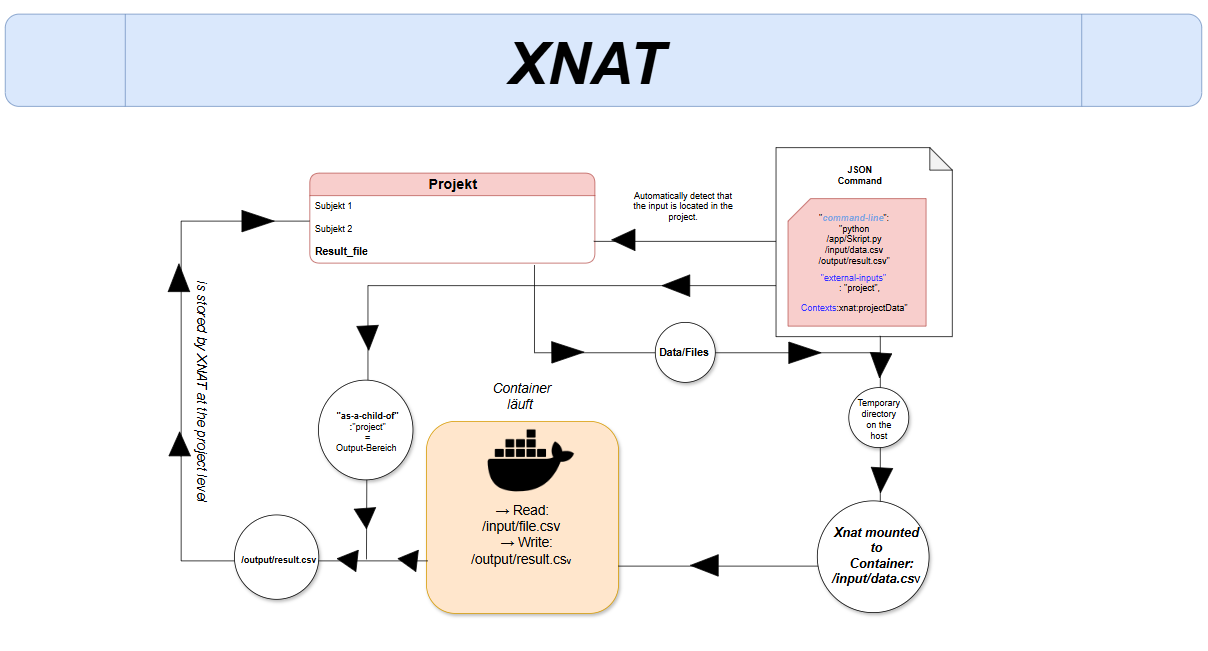
\includegraphics[width=1\linewidth]{en/content/WO.png}
    \caption{XNAT Workflow Data with the Container  }
    \label{fig:enter-label}
\end{figure}
In my view the script works amazing if the main goal wasn't to launch only one container,or to launch in every context a container. but still the processing files time is going to be extreme long for huge projects. In my case i have tested to launch for every singles files in my project ( around 700) a container and it took me 4 min in general to proceed all the files. Having more than one container in multiple context will reduced the time consumed.

Overall it is clear that while XNAT’s workflow enables containerized processing by mounting or copying data to temporary directories on the host system, but the truth that a huge amount of data can slow down or bug the system. And this approach may introduce limitations related to storage or system resources, even when datasets are not exceptionally large. however, persistent failures suggest that additional factors, beyond dataset size or file limits, could be influencing processing success.